\chapter{Voraussetzungen}
Getestet wurde diese Installation auf einer frischen Installation von Debian. Dieses Installationsskript ist auch ausschließlich unter Distributionen lauffähig, die \emph{apt-get} verwenden.

\chapter{Installation eines Webservers}
\paragraph{LAMP}
LAMP steht für \emph{Linux, Apache, MySQL, PHP} und stellt die Basis eines einfachen Webservers dar.\par

Die Installation wird mit 

\begin{lstlisting}
	sudo sh installLAMP.sh
\end{lstlisting}

begonnen.

\begin{figure}[!ht]
	\centering
	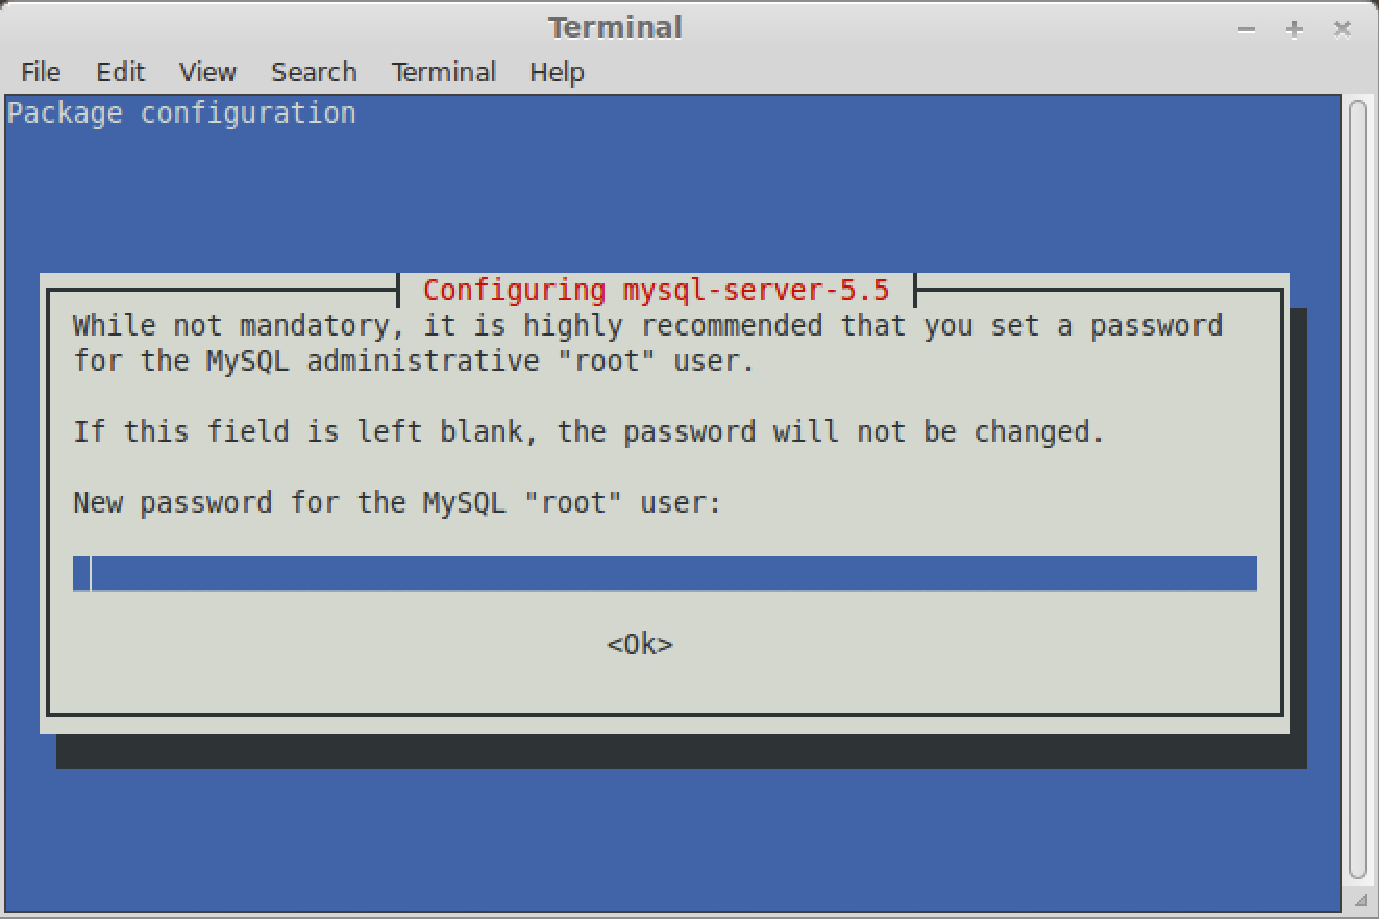
\includegraphics[width=15cm]{fig/configuring_mysql}
	\caption{Eingabe des root Passworts für die MySQL Datenbank}
\end{figure}

\begin{figure}[!ht]
	\centering
	\includegraphics[width=15cm]{fig/configuring_phpmyadmin}
	\caption{Eingabe des root Passworts für phpmyadmin}
\end{figure}

